\documentclass[dvipdfmx,fleqn,article]{jlreq}
\usepackage{graphicx}
\usepackage{bxtexlogo}
\usepackage{fancyhdr} % ヘッダーとフッターのカスタマイズ用
\usepackage{amsmath} % Add this line to include the amsmath package
\usepackage{placeins} 
\usepackage{float}
\usepackage{enumitem}
\usepackage{listings}
\usepackage{xcolor}

\lstdefinelanguage{CSharp}{
  morekeywords={abstract, event, new, struct, as, explicit, null, switch, base, extern, object, this, bool, false, operator, throw, break, finally, out, true, byte, fixed, override, try, case, float, params, typeof, catch, for, private, uint, char, foreach, protected, ulong, checked, goto, public, unchecked, class, if, readonly, unsafe, const, implicit, ref, ushort, continue, in, return, using, decimal, int, sbyte, virtual, default, interface, sealed, volatile, delegate, internal, short, void, do, is, sizeof, while, double, lock, stackalloc, else, long, static, enum, namespace, string},
  sensitive=true,
  morecomment=[l]{//},
  morecomment=[s]{/*}{*/},
  morestring=[b]",
  morestring=[b]',
  morestring=[b]"""
}

\lstset{
  language=CSharp,
  basicstyle=\ttfamily\footnotesize,
  commentstyle=\color{gray},
  numbers=left,
  numberstyle=\tiny\color{gray},
  stepnumber=1,
  numbersep=5pt,
  backgroundcolor=\color{white},
  showspaces=false,
  showstringspaces=false,
  showtabs=false,
  frame=single,
  tabsize=2,
  captionpos=b,
  breaklines=true,
  breakatwhitespace=false,
  escapeinside={(*@}{@*)},
  caption={リスト \thelstlisting: \lstname}
}

\renewcommand{\lstlistingname}{リスト}

\title{ソフトウェアアーキテクチャ 特論 期末レポート}
\author{M24J4045A 中邑熙正}
\date{\today}

\begin{document}
\thispagestyle{empty} % 表紙にページ番号を表示しない
\maketitle
\newpage

\tableofcontents
\newpage



\section{はじめに}
\subsection{レポートの目的}
このレポートの目的は、ソフトウェアアーキテクチャ特論の授業で学んだ知識をもとに、
Webアプリケーションとゲームの両方に適用し、その適用事例を整理することである。
\subsection{開発したソフトウェアの概要}
\subsubsection{Webアプリケーション}
今回作成したのはn年日記というWebアプリケーションである。
n年日記は、ユーザが日記を書くことができるWebアプリケーションである。
n年日記の開発に当たって、10年日記\cite{website1}というアプリケーションを参考にした。
10年日記は通常の日記アプリとは異なり、ある日付の未来の日記を一覧表示することができる。
例えば、2021年1月1日の日記を書くと、2022年1月1日、2023年1月1日、・・・、
2030年1月1日の日記も一覧表示される。
しかし10年日記を利用していてその日付の過去の日記が表示されないことが不便だと感じた。
むしろ、その日付の過去の日記を見返すことができる方が便利だと考えたため、
n年日記では、その日付の過去の日記が一覧表示されるように改良したアプリケーションを作成する。

\subsubsection{ゲーム}
今回扱うゲームは、増殖する細菌・微生物たちを操作して、敵の微生物を倒す2Dアクションゲームである。
以前から個人開発していたものであり、
今回はこのゲームをソフトウェアアーキテクチャの観点から再設計する。

\section{Ruby on Rails}
n年日記の開発では、フレームワークにRuby on Railsを用いている。
Ruby on Rails(以下、Rails)は、MVCアーキテクチャに基づくWebアプリケーションフレームワークであり、
開発の効率性を向上させるための機能が充実している。
以下に、Railsの特徴をいくつか紹介する。
\subsection{MVCアーキテクチャ}
Rails は Model-View-Controller(MVC)アーキテクチャ を採用しており、
Webアプリケーションの構造を明確に分離することで、拡張性と保守性を向上させている。

Model(モデル) はアプリケーションのデータやビジネスロジックを管理する。
View(ビュー) はユーザーとのインターフェースを担当する。
Controller(コントローラ) は Model と View の橋渡しを行い、リクエストの処理とデータの制御を行う。
この分割により、各コンポーネントが独立して開発・変更できるため、スケーラビリティが向上する。例えば、データベースのスキーマを変更する場合でも、View のコードには影響を与えずに Model 層のみを修正すればよい。


MVCアーキテクチャにおけるデータの流れを図\ref{fig:MVC}に示す。

\begin{figure}[H]
    \centering
    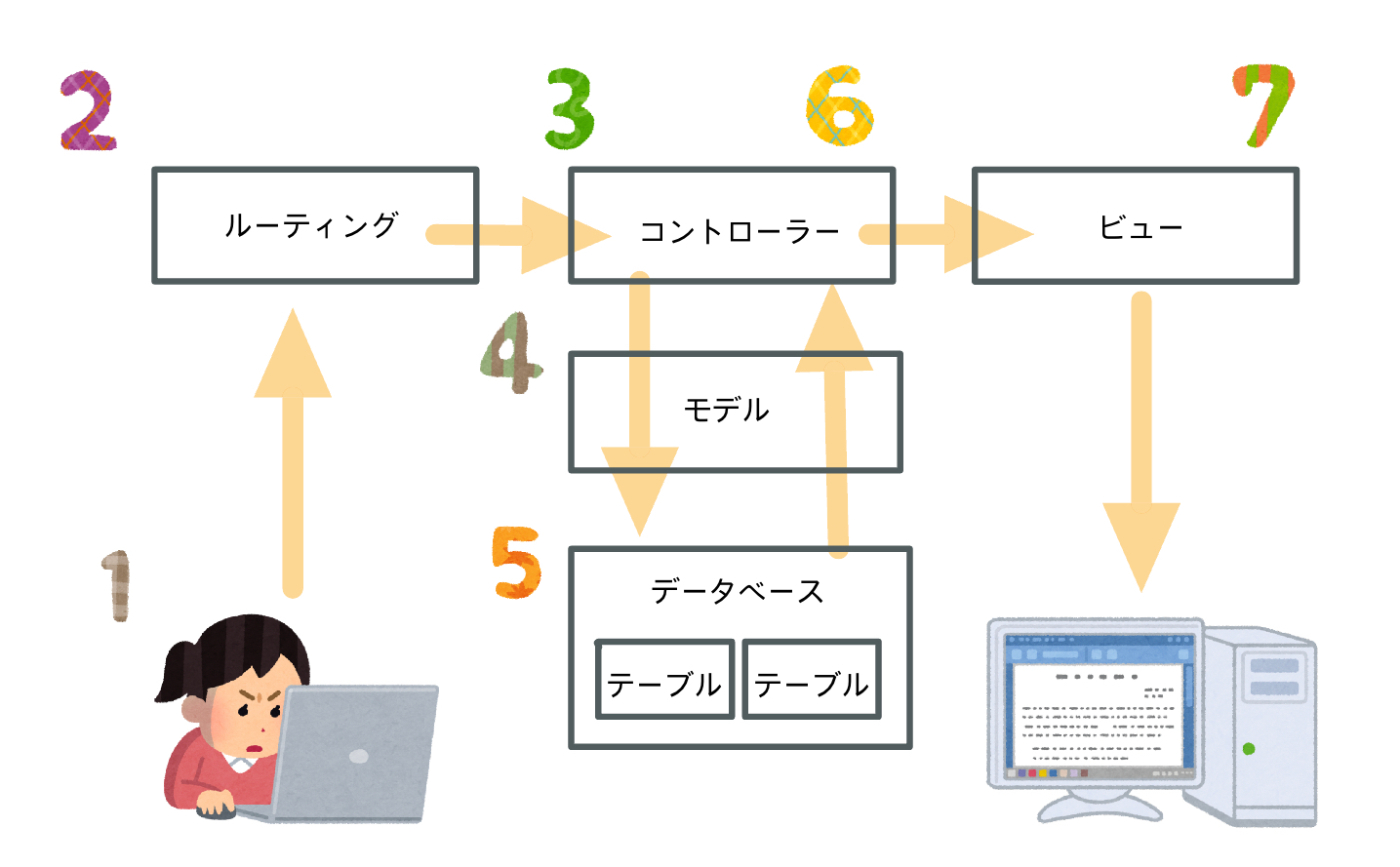
\includegraphics[width=1\textwidth]{figures/MVC.png}
    \caption{MVCアーキテクチャ}
    \label{fig:MVC}
\end{figure}

アプリケーションの処理は、ユーザーの操作によるリクエストの送信から始まる。
まず、ルーティングによってリクエストが解析され、適切なコントローラーに振り分けられる。
コントローラーはアプリケーションの処理を制御し、必要に応じてモデルにデータの取得を依頼する。
モデルはデータの管理とデータベースとのやり取りを担当し、コントローラーからの要求に応じてデータを
取得または加工し、それを返す。コントローラーは受け取ったデータをビューに渡し、
ビューはそのデータをもとに画面を生成し、ユーザーに表示する。
MVCを採用することで、役割が明確に分かれ、コードの管理が容易になり、
開発の拡張性やメンテナンス性が向上する。



% \subsection{Convention over Configuration(設定より規約)}
% 「設定より規約」 という思想で、一般的な Web アプリ開発のパターンを規約として定め、開発者が細かい設定をせずに済むようにする。
% 例えば、モデル名 User を定義すると、Rails は自動的に users テーブルを参照するようになっており、設定なしでデータベースとの連携が可能。
% \subsection{DRY(Don't Repeat Yourself)の原則}
% 同じコードを繰り返し書かず、再利用可能な形で設計する。
\subsection{データベース管理とマイグレーション}
Rails は ActiveRecord を用いた ORM(オブジェクト・リレーショナル・マッピング) により、データベースとのやりとりを抽象化している。これにより、開発者は SQL を直接書かずにデータを操作できる。 また、マイグレーション機能を活用することで、データベースの構造変更が簡単に行える。
データベースの変更履歴をバージョン管理できるため、
どのような変更が行われたのかを記録し、必要に応じてロールバックも可能である。
またデータベースの知識がなくても構造変更ができるため、Rails 側で rails db:migrate を実行するだけで、
自動的にテーブルを作成・更新できる。
このようにRails のデータベース管理機能は開発のスピードを向上させつつ、システムの一貫性を保つ設計になっている。

\subsection{Active Record}
Active Recordとは、RailsのMVCアーキテクチャの中のModelに相当する部分である。
Active Recordは、データベースとのやり取りを行うためのクラスであり、
データベースのテーブルと1対1で対応している。
Active Recordを用いることで、データベースの操作を簡単に行うことができる。
DBとのやり取りを抽象化することで、データベースの変更に強くなる。


\section{Webアプリケーション n年日記}
n年日記の開発では、フレームワークにRuby on Rails、データベースにSQLiteを用いた。

\subsection{設計}
DB設計を表\ref{tab:diary_entries}に示す。
\begin{table}[h]
    \centering
    \caption{\texttt{diary\_entries} テーブルのカラム定義}
    \label{tab:diary_entries}
    \begin{tabular}{|l|l|l|}
        \hline
        \textbf{カラム名} & \textbf{データ型} & \textbf{説明} \\ \hline
        \texttt{id} & 整数型 (主キー) & 各日記エントリの一意の識別子 \\ \hline
        \texttt{content} & テキスト型 & 日記の内容 \\ \hline
        \texttt{date} & 日付型 & 日記の記録日 \\ \hline
        \texttt{created\_at} & 日時型 & レコードが作成された日時 \\ \hline
        \texttt{updated\_at} & 日時型 & レコードが最後に更新された日時 \\ \hline
    \end{tabular}
\end{table}

\noindent
上記のテーブルは、日記エントリの情報を管理するために使用される。
\texttt{id} は各エントリを一意に識別するための主キーであり、
\texttt{date} カラムには日記の記録日を格納する。\texttt{created\_at}
 および \texttt{updated\_at} は、データの作成・更新時刻を管理する。



\subsection{実装}

実装の一部を示す。
モデルとしてDiaryEntryクラスをリスト\ref{lst:DiaryEntry}に示す。

\begin{lstlisting}[language=CSharp, caption=DiaryEntryクラス, label={lst:DiaryEntry}]
class DiaryEntry < ApplicationRecord
  def self.fetch_entries(selected_date, n_years)
    (0..n_years-1).map do |years_ago|
      target_date = selected_date - years_ago.years
      find_or_initialize_by(date: target_date)
    end.reverse
  end
end
  
\end{lstlisting}


コントローラにあたるDiaryEntriesController は、日記エントリの表示、作成、編集、更新を担当している。
以下に、主要なアクションの説明を示す。

\begin{itemize}
    \item \textbf{index}: 指定した日付に基づいて過去n年分の日記を表示
    \item \textbf{new}: 新規日記作成画面を表示
    \item \textbf{create}: 新しい日記エントリを作成
    \item \textbf{edit}: 日記エントリの編集画面を表示
    \item \textbf{update}: 日記エントリを更新
\end{itemize}

DiaryEntriesControllerクラスの実装をリスト\ref{lst:DiaryEntryController}に示す。
\begin{lstlisting}[language=CSharp, caption=DiaryEntryControllerクラス, label={lst:DiaryEntryController}]
  class DiaryEntriesController < ApplicationController
  # メイン画面(指定した日付に基づいて過去n年分の日記を表示)
  def index
    # selected_dateが指定されていない場合、今日の日付を使用
    @selected_date = params[:selected_date] ? Date.parse(params[:selected_date]) : Date.today
  
    # start_dateが指定されていない場合、selected_dateの月の開始日を使用
    @start_date = params[:start_date] ? Date.parse(params[:start_date]) : @selected_date.beginning_of_month
  
    @n_years = 5 # 過去何年分表示するか
  
    # 過去n年分の日記データを取得
    @diary_entries = DiaryEntry.fetch_entries(@selected_date, @n_years)
  end

  # 日記の新規作成画面
  def new
    @diary_entry = DiaryEntry.new(date: params[:date])
  end

  # 日記の作成
  def create
    @diary_entry = DiaryEntry.new(diary_entry_params)
    if @diary_entry.save
      redirect_to diary_entries_path(selected_date: @diary_entry.date), notice: '日記が作成されました。'
    else
      flash.now[:alert] = '日記の作成に失敗しました。'
      flash.now[:alert] += @diary_entry.errors.full_messages.join(", ")
      render :new
    end
  end

  # 日記の編集画面
  def edit
    @diary_entry = DiaryEntry.find(params[:id])
  end

  # 日記の更新
  def update
    @diary_entry = DiaryEntry.find(params[:id])
    if @diary_entry.update(diary_entry_params)
      redirect_to diary_entries_path(selected_date: @diary_entry.date), notice: '日記が更新されました。'
    else
      flash.now[:alert] = '日記の更新に失敗しました。'
      flash.now[:alert] += @diary_entry.errors.full_messages.join(", ")
      render :edit
    end
  end

  private

  def diary_entry_params
    params.require(:diary_entry).permit(:content, :date)
  end
end
\end{lstlisting}

ビューとしてindex.html.erbをリスト\ref{lst:index}に示す。

\begin{lstlisting}[language=CSharp, caption=index.html.erb, label={lst:index}]
<h1>n年日記</h1>
<div class="container">
  <div class="left-column">
    <div class="diary-entries">
      <h2><%= @selected_date.strftime('%Y年 %m月 %d日') %> の過去<%= @n_years %>年分</h2>
      <% @diary_entries.reverse.each do |entry| %>
        <div id="diary-entry-<%= entry.id %>" class="diary-entry">
          <p><%= entry.date.strftime('%Y年 %m月 %d日 (%A)') %></p>
          <% if entry.persisted? && entry.content.present? %>
            <!-- 日記が存在し、内容がある場合 -->
            <p><%= entry.content %></p>
            <%= link_to '編集', edit_diary_entry_path(entry), class: 'edit-link', data: { id: entry.id } %>
          <% elsif entry.persisted? %>
            <!-- 日記が存在するが、内容がない場合 -->
            <%= link_to '編集', edit_diary_entry_path(entry), class: 'edit-link', data: { id: entry.id } %>
          <% else %>
            <!-- 日記が存在しない場合 -->
            <%= link_to '新規作成', new_diary_entry_path(date: entry.date), class: 'edit-link', data: { id: entry.id } %>
          <% end %>
        </div>
      <% end %>
    </div>
  </div>

  <div class="right-column">
    <div class="calendar">
      <%= month_calendar(start_date: @start_date, previous_label: nil, next_label: nil) do |date| %>
        <div class="day">
          <% if date == @selected_date %>
            <!-- 選択中の日付 -->
            <strong class="selected-date"><%= link_to date.day, diary_entries_path(selected_date: date) %></strong>
          <% elsif date == Date.today %>
            <!-- 今日の日付 -->
            <span class="today-date"><%= link_to date.day, diary_entries_path(selected_date: date) %></span>
          <% else %>
            <!-- 通常の日付 -->
            <%= link_to date.day, diary_entries_path(selected_date: date) %>
          <% end %>
        </div>
      <% end %>
    </div>

    <div class="navigation">
      <%= link_to 'Previous Year', diary_entries_path(start_date: @start_date.beginning_of_year - 1.year, selected_date: @selected_date) %> |
      <%= link_to 'Previous Month', diary_entries_path(start_date: @start_date.beginning_of_month - 1.month, selected_date: @selected_date) %> |
      <%= link_to 'Today', diary_entries_path(start_date: Date.today.beginning_of_month, selected_date: Date.today) %> |
      <%= link_to 'Next Month', diary_entries_path(start_date: @start_date.beginning_of_month + 1.month, selected_date: @selected_date) %> |
      <%= link_to 'Next Year', diary_entries_path(start_date: @start_date.beginning_of_year + 1.year, selected_date: @selected_date) %>
    </div>
  </div>
</div>
    
\end{lstlisting}

図\ref{fig:Home}に示すのは、n年日記アプリケーションのホーム画面である。このアプリケーションは、ユーザーが日記を記録し、過去の同じ日付の日記を一覧表示することができるWebアプリケーションである。

\begin{figure}[H]
    \centering
    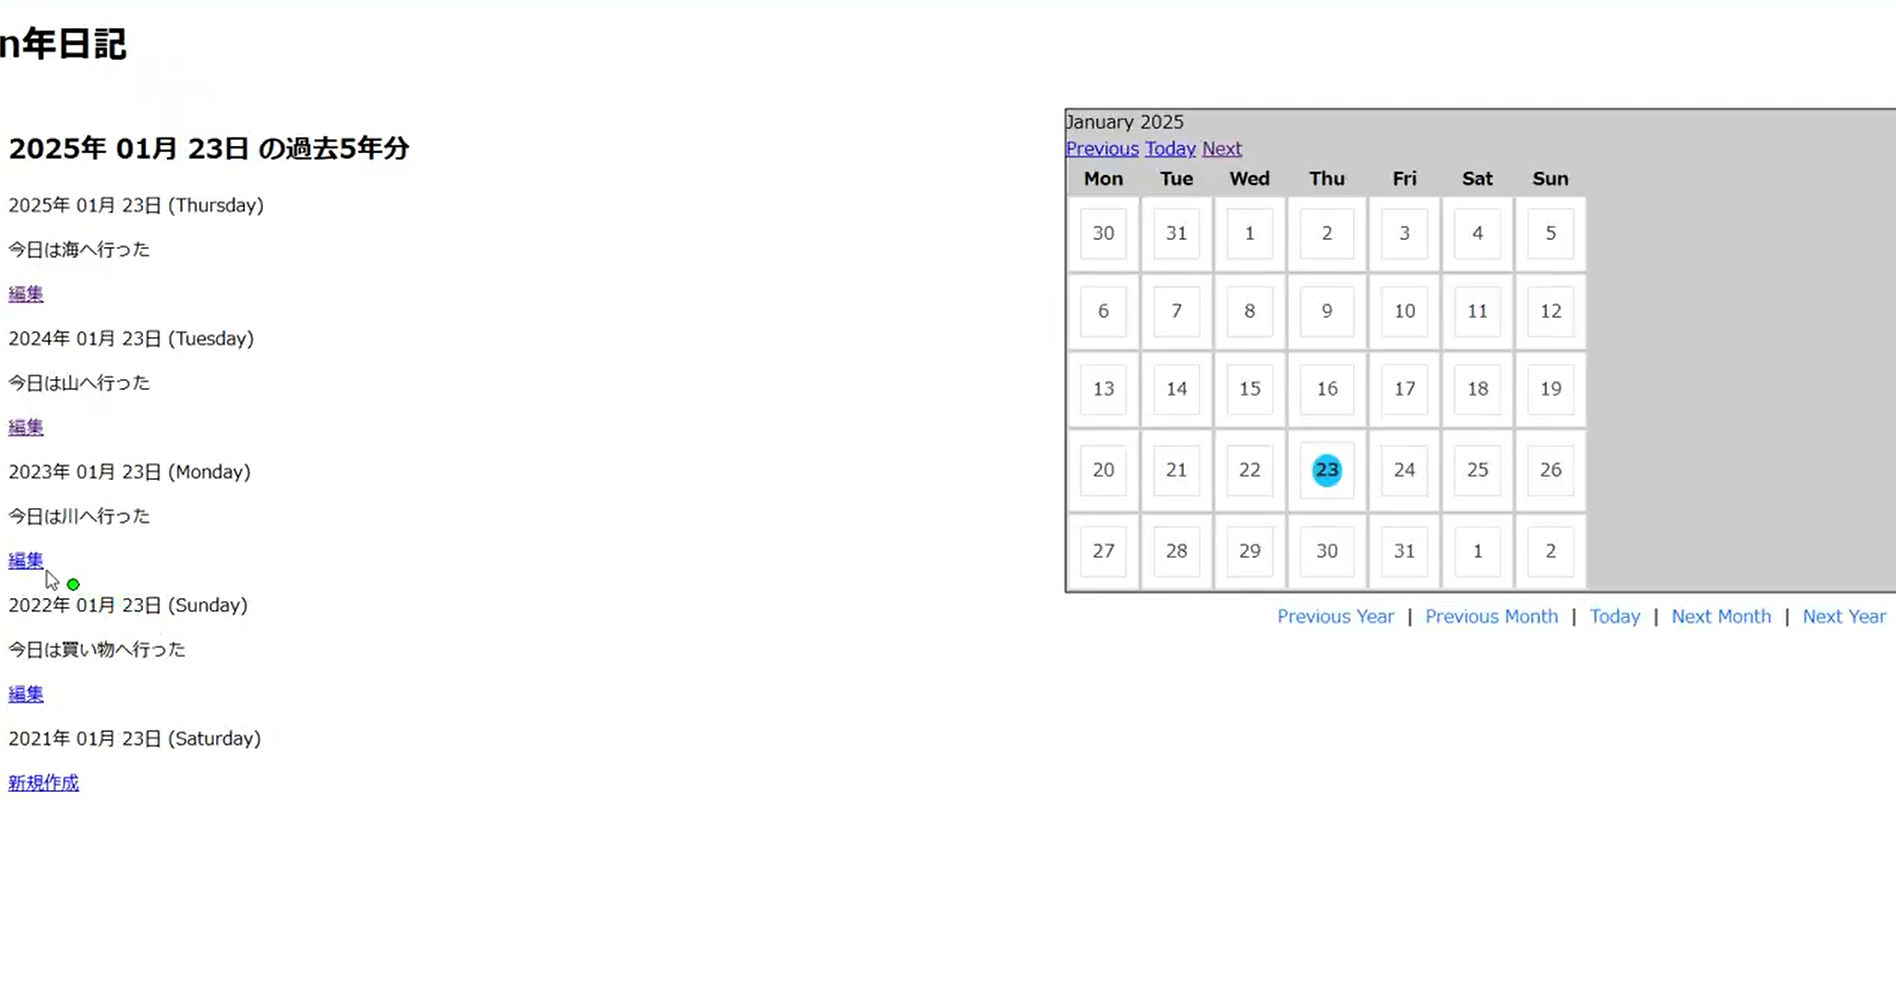
\includegraphics[width=1\textwidth]{figures/Home.png}
    \caption{ホーム画面}
    \label{fig:Home}
\end{figure}

ホーム画面は大きく分けて左カラムと右カラムの2つのセクションに分かれている。

左カラムには、選択された日付の過去n年分の日記エントリが表示される。各日記エントリは以下の情報を含む。

\begin{itemize}
    \item 日記の記録日
    \item 日記の内容(存在する場合)
    \item 編集リンク(内容が存在する場合)
    \item 新規作成リンク(内容が存在しない場合)
\end{itemize}

ユーザーは、日記エントリの内容を確認し、必要に応じて編集することができる。また、日記が存在しない場合は、新規作成リンクをクリックして新しい日記を作成することができる。

右カラムには、カレンダーとナビゲーションリンクが表示される。

カレンダーは、選択された月の日付を表示し、ユーザーが特定の日付を選択できるようにする。カレンダーの日付は以下のように表示される。

\begin{itemize}
    \item 選択中の日付は太字で強調表示される。
    \item 今日の日付は特別なスタイルで表示される。
    \item 通常の日付はリンクとして表示され、クリックするとその日付の日記エントリが表示される。
\end{itemize}

ナビゲーションリンクは、ユーザーが異なる期間の日記エントリを簡単に表示できるようにする。以下のリンクが含まれる。

\begin{itemize}
    \item 前年の表示
    \item 前月の表示
    \item 今日の日付の表示
    \item 次月の表示
    \item 次年の表示
\end{itemize}

これらのリンクを使用することで、ユーザーは簡単に異なる期間の日記エントリを表示し、過去の日記を振り返ることができる。

このように、n年日記アプリケーションは、ユーザーが日記を記録し、過去の日記を簡単に参照できるように設計されている。ユーザーは、日記の内容を編集したり、新しい日記を作成したりすることができ、日々の出来事を記録し続けることができる。




% \begin{figure}[H]
%     \centering
%     \includegraphics[width=1\textwidth]{figures/New.png}
%     \caption{日記新規作成画面}
%     \label{fig:New}
% \end{figure}


% \begin{figure}[H]
%     \centering
%     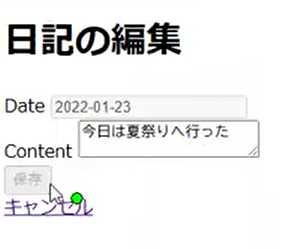
\includegraphics[width=0.5\textwidth]{figures/Edit.png}
%     \caption{日記編集画面}
%     \label{fig:Edit}
% \end{figure}























\section{ゲーム}
今回扱うゲームは、増殖する細菌・微生物たちを操作して、敵の微生物を倒す2Dアクションゲームである。
ゲームエンジンであるUnityとC\#を用いて開発した。

\subsection{設計}
ソフトウェアアーキテクチャの設計原則に基づいて、ゲームの設計を行うにあたって、
ゲームが抱えている課題を解決するためにデザインパターンを適用する。
今回はGoFの23種類のデザインパターンの中から、StrategyパターンとObserverパターンを適用した。
デザインパターンについては\cite{book1}を参考にした。
\subsubsection{Strategyパターン}
Strategyパターンは、一連のアルゴリズムを定義してカプセル化し交換できるようにするデザインパターンである。
Strategyパターンを使うと、アルゴリズムを利用するクライアントとは独立して、
アルゴリズムを変更することができる。
このゲームでは、キャラクターごとに異なる攻撃パターンを持っている。
例えば、敵に体当たりした時にダメージを与えるだけのキャラクターや、
攻撃時に自爆して敵を道連れにするキャラクターがいる。
Strategyパターンを用いることで、キャラクターごとに異なる攻撃パターンを実装することができる。
ここでは、Strategyパターンを用いてキャラクターの攻撃パターンを実装する方法を説明する。



今回作成したStrategyパターンに関連するクラス図を図\ref{fig:Strategy}に示す。
\begin{figure}[H]
    \centering
    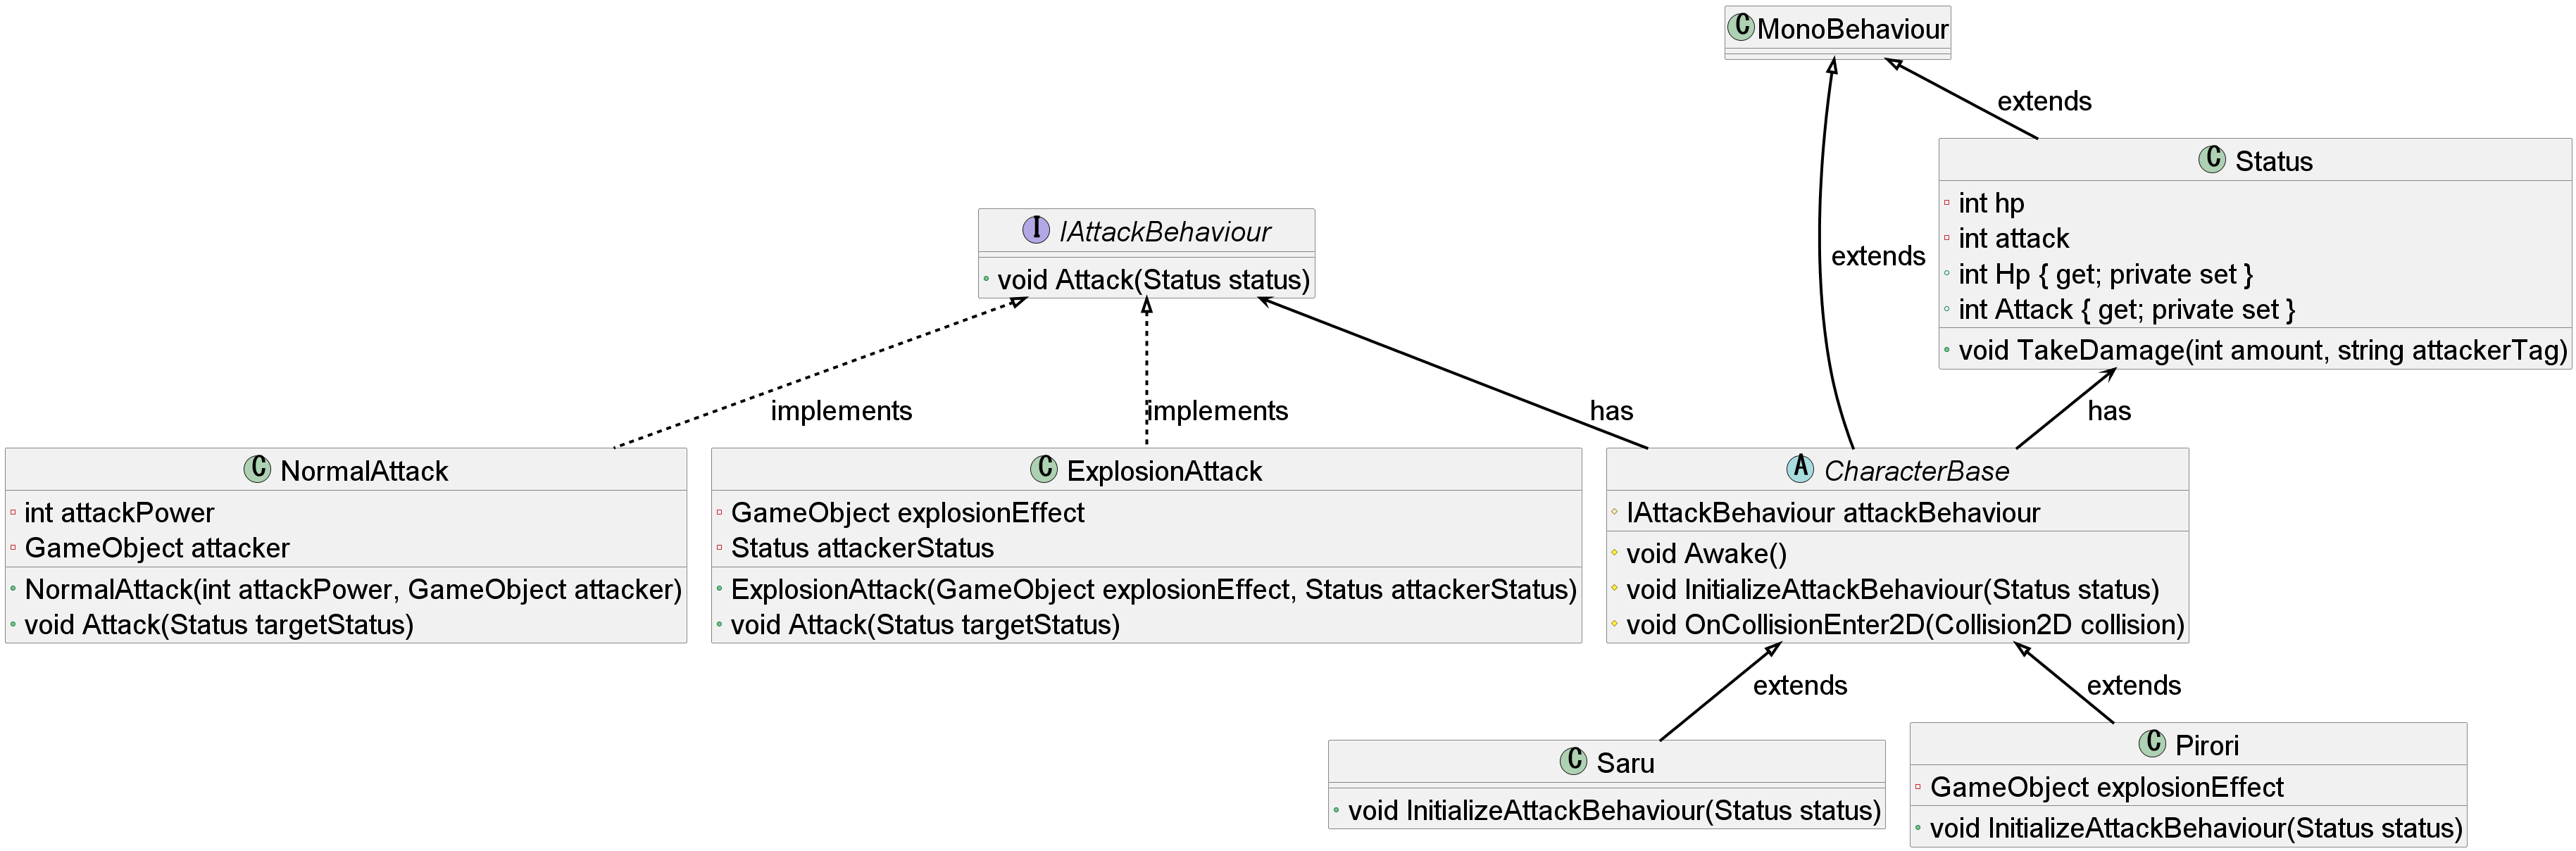
\includegraphics[width=1\textwidth]{figures/Strategy.png}
    \caption{Strategyパターンのクラス図}
    \label{fig:Strategy}
\end{figure}

各クラスの説明を表\ref{table:Strategy}に示す。

\begin{table}[H]
    \centering
    \begin{tabular}{|c|c|}
        \hline
        クラス名 & 役割 \\
        \hline
        IAttackBehaviour & 攻撃の振る舞いを定義するインターフェース \\
        \hline
        NormalAttack & 通常攻撃の振る舞いを実装するクラス \\
        \hline
        ExplosionAttack & 爆発攻撃の振る舞いを実装するクラス \\
        \hline
        CharacterBase & キャラクターの基底クラス(抽象クラス) \\
        \hline
        Saru & 通常攻撃を行うキャラクターのクラス \\
        \hline
        Pirori & 爆発攻撃を行うキャラクターのクラス \\      
        \hline
        Status & キャラクターのステータスを管理するクラス \\
        \hline
        MonoBehaviour & Unityのすべてのスクリプトの基本クラス。 \\
        & このクラスを継承することでStart(), Awake(), OnCollisionEnter2D()\\
        & などのUnityが提供するメソッドを使用できるようになる。 \\
        \hline
    \end{tabular}
    \caption{Strategyパターンに関連する各クラスの役割}
    \label{table:Strategy}  
\end{table}


まず攻撃の振る舞いを定義するIAtttackBehaviorインターフェースを定義する。
IAttackBehaviorを実装したクラスとして、通常攻撃の振る舞いを実装するNormalAttackクラス, 
爆発攻撃の振る舞いを実装するExplosionAttackクラスを定義する。
続いて、キャラクターの基底クラスとなるCharacterBaseクラスを定義し、
AttackBehavior型のインスタンス変数attackBehaviourを保持させる。
CharacterBaseクラスを継承したキャラクタークラスとして、SaruクラスとPiroriクラスを定義する。
これらのクラスの初期化の際に任意の攻撃パターンを設定する。
今回はSaruクラスはNormalAttackクラス、PiroriクラスはExplosionAttackクラスを攻撃パターンとして設定するものとする。
攻撃実行時はattackBehaviourのAttackメソッドを呼び出すことで、
キャラクターに設定された攻撃パターンが実行される。
Attackメソッドの具体的な処理はNormalAttackクラスとExplosionAttackクラスに委譲されている。
もし攻撃パターンを変更したい場合は、SetAttackBehaviorメソッドを呼び出すことで、
attackBehaviourの中身を変更することができる。\\
また、Statusクラスはキャラクターのステータスを管理するクラスである。
ここではインスタンス変数hp, attackやTakeDamageメソッドといったダメージ関連処理のみを記述している。
加えて、MonoBehaviourクラスはUnityのすべてのスクリプトの基本クラスであり、
キャラクターがゲーム内オブジェクトとして動作するために継承する必要がある。

\subsubsection{Observerパターン}
Observerパターンとは、オブジェクトの状態変化を他のオブジェクトに通知するためのデザインパターンである。
Observerパターンを用いることで、オブジェクト間の依存関係を減らすことができる。
このゲームでは、プレイヤー側のキャラクターは選択して動かせる。
しかし、選択されているキャラクターの中で、あるキャラクターが死んでしまった場合、
その集団を移動させる時にnullを参照してしまい、エラーが発生してしまう。
そのため、そのキャラクターを即座に配列から削除する処理を実装しなければならない。
そこで、Observerパターンを用いて、キャラクターの死亡イベントを購読することで、
死亡したキャラクターを配列から削除する処理を実装する。

今回実装するObserverパターンのクラス図を図\ref{fig:ObserverClassDiagram}に示す。
\begin{figure}[H]
    \centering
    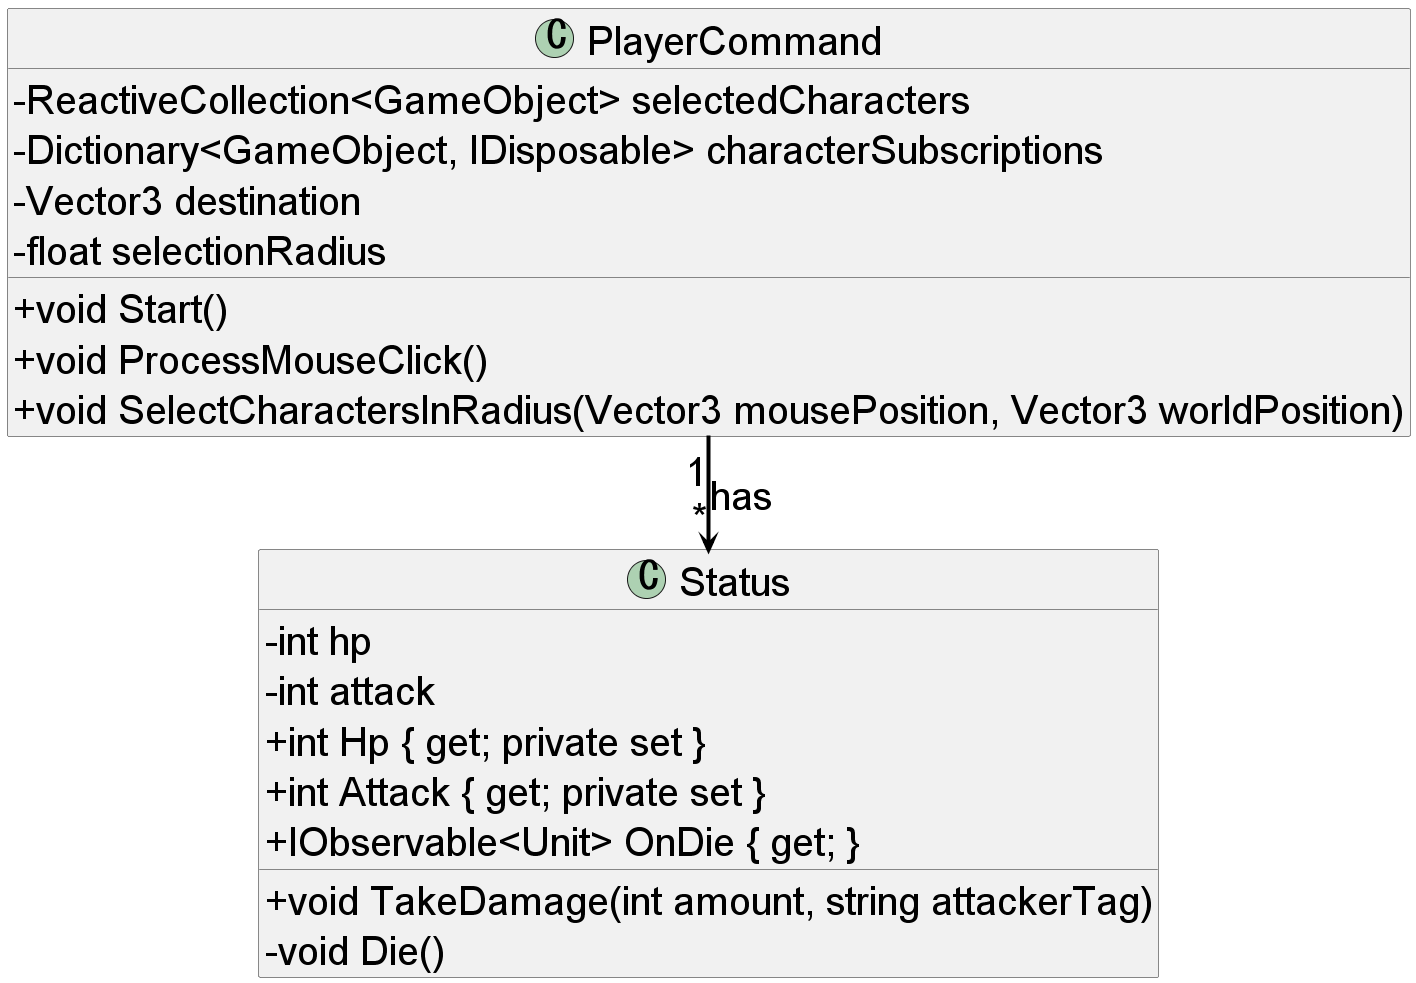
\includegraphics[width=0.7\textwidth]{figures/ObserverClassDiagram.png}
    \caption{Observerパターンのクラス図}
    \label{fig:ObserverClassDiagram}
\end{figure}

PlayerCommandクラスは、プレイヤーが選択したキャラクターを操作するためのクラスである。
レイヤーがクリックした位置にあるキャラクターを選択し、
その次にクリックした位置に移動させることができる。
Statusクラスはキャラクターのステータスを管理するクラスである。
ここでは両クラスともに、死亡イベントに関連する処理のみを記述し、それ以外の処理は省略している。

また、今回実装するObserverパターンのシーケンス図を図\ref{fig:Observer}に示す。
\begin{figure}[H]
    \centering
    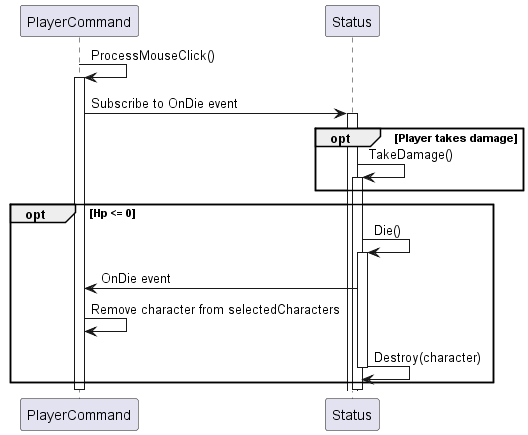
\includegraphics[width=1\textwidth]{figures/Observer.png}
    \caption{Observerパターンのシーケンス図}
    \label{fig:Observer}
\end{figure}

図\ref{fig:Observer}に示すシーケンス図は、Observerパターンを用いたキャラクターの死亡イベントの管理を表している。
本シーケンス図では、PlayerCommandクラスがキャラクターの死亡イベントを購読し、
キャラクターが死亡した際にselectedCharactersコレクションから削除する処理を実装している。

\begin{enumerate}
    \item \textbf{マウスクリックの処理} PlayerCommandクラスのProcessMouseClickメソッドが呼び出され、プレイヤーがクリックした位置にあるキャラクターを選択する。
    \item \textbf{死亡イベントの購読} PlayerCommandクラスがStatusクラスのOnDieイベントを購読することで、キャラクターが死亡した際に通知を受け取る準備をする。
    \item \textbf{ダメージの受け取り} キャラクターが攻撃を受けた場合、StatusクラスのTakeDamageメソッドが呼び出され、キャラクターのHPが減少する。
    \item \textbf{HPのチェックと死亡処理} TakeDamageメソッド実行後、キャラクターのHPが0以下になった場合、StatusクラスのDieメソッドが実行され、OnDieイベントが発行される。
    \item \textbf{死亡イベントの発行} Dieメソッド内でOnDieイベントが発行され、PlayerCommandクラスに通知される。
    \item \textbf{キャラクターの削除} PlayerCommandクラスはOnDieイベントを受け取ると、死亡したキャラクターをselectedCharactersコレクションから削除し、さらにStatusクラスでDestroyメソッドを呼び出してキャラクターを削除する。
\end{enumerate}

このようにObserverパターンを利用することで、PlayerCommandクラスはキャラクターの死亡を監視し、死亡時に適切な処理を実行できる仕組みを構築している。



\subsection{実装}

\subsubsection{Strategyパターンの実装}
ここではStrategyパターンに関連するクラスの実装を示す。
まず攻撃の振る舞いを定義するIAtttackBehaviorインターフェースをリスト\ref{lst:IAttackBehaviour}に示す。
\begin{lstlisting}[language=CSharp, caption=IAttackBehaviourインターフェース, label={lst:IAttackBehaviour}]
public interface IAttackBehaviour
{
    void Attack(Status status);
}
\end{lstlisting}

IAttackBehaviorを実装したクラスとして、通常攻撃の振る舞いを実装するNormalAttackクラス, 
爆発攻撃の振る舞いを実装するExplosionAttackクラスを
それぞれリスト\ref{lst:NormalAttack}とリスト\ref{lst:ExplosionAttack}に示す。

\begin{lstlisting}[language=CSharp, caption=NormalAttackクラス, label={lst:NormalAttack}]
using UnityEngine;

/// <summary>
/// 通常攻撃
/// </summary>
public class NormalAttack : IAttackBehaviour
{
    private int attackPower;
    private GameObject attacker;

    public NormalAttack(int attackPower, GameObject gameObject)
    {
        this.attackPower = attackPower;
        this.attacker = gameObject;
    }

    public void Attack(Status targetStatus)
    {
        if (targetStatus != null && attacker.tag != targetStatus.gameObject.tag)
        {
            targetStatus.TakeDamage(attackPower, attacker.tag);
        }
    }
}
\end{lstlisting}

\begin{lstlisting}[language=CSharp, caption=ExplosionAttackクラス, label={lst:ExplosionAttack}]
using UnityEngine;
using UnityEngine.AddressableAssets;
using UnityEngine.ResourceManagement.AsyncOperations;

/// <summary>
/// ぶつかった敵とともに爆発
/// </summary>
public class ExplosionAttack : IAttackBehaviour
{
    private GameObject explosionEffect;
    private Status attackerStatus;
    private const string explosionEffectAddress = "省略";

    public ExplosionAttack(Status attackerStatus)
    {
        this.attackerStatus = attackerStatus;
        LoadExplosionEffect();
    }

    private void LoadExplosionEffect()
    {
        // 省略
    }

    private void OnExplosionEffectLoaded(AsyncOperationHandle<GameObject> obj)
    {
        // 省略
    }

    public void Attack(Status targetStatus)
    {
        if (targetStatus != null && explosionEffect != null)
        {
            GameObject.Instantiate(explosionEffect, targetStatus.transform.position, Quaternion.identity);
            GameObject.Destroy(targetStatus.gameObject); // 敵を破壊
            GameObject.Destroy(attackerStatus.gameObject); // 自分自身も破壊
        }
    }
}
\end{lstlisting}


次に、キャラクターの基底クラスとなるCharacterBaseクラスをリスト\ref{lst:CharacterBase}に示す。
\begin{lstlisting}[language=CSharp, caption=CharacterBaseクラス, label={lst:CharacterBase}]
using UnityEngine;

/// <summary>
/// キャラクターの基底クラス
/// </summary>
public abstract class CharacterBase : MonoBehaviour
{
    protected IAttackBehaviour attackBehaviour;
    private Status status;

    /// <summary>
    /// 開始時に呼び出されるメソッド
    /// </summary>
    protected void Awake()
    {
        status = GetComponent<Status>();
        if (status != null)
        {
            InitializeAttackBehaviour(status);
        }
        else
        {
            Debug.LogError("Status component not found on " + gameObject.name);
        }
    }

    /// <summary>
    /// 攻撃パターンを初期化するメソッド
    /// </summary>
    protected abstract void InitializeAttackBehaviour(Status status);

    protected virtual void OnCollisionEnter2D(Collision2D collision)
    {
        if (collision.gameObject.CompareTag("Enemy"))
        {
            var targetStatus = collision.gameObject.GetComponent<Status>();
            if (targetStatus != null)
            {
                attackBehaviour.Attack(targetStatus);
            }
        }
    }

    /// <summary>
    /// 攻撃パターンを設定するメソッド
    /// </summary>
    public void SetAttackBehaviour(IAttackBehaviour attackBehaviour)
    {
        this.attackBehaviour = attackBehaviour;
    }
}
\end{lstlisting}    

SaruクラスとPiroriクラスの初期化の際に、
SaruクラスはNormalAttackクラス、PiroriクラスはExplosionAttackクラスを攻撃パターンとして設定する。
実装をリスト\ref{lst:Saru}とリスト\ref{lst:Pirori}に示す。
Strategyパターンを適用しているため、
コメントアウトしている部分を有効にすることで攻撃パターンを変更することができる。
\begin{lstlisting}[language=CSharp, caption=Saruクラス, label={lst:Saru}]
public class Saru : CharacterBase
{
    protected override void InitializeAttackBehaviour(Status status)
    {
        SetAttackBehaviour(new NormalAttack(status.Attack, gameObject));
        // 例えば以下のように書き換えると攻撃パターンを爆発攻撃に変更することができる
        // SetAttackBehaviour(new ExplosionAttack(status));
    }
}
\end{lstlisting}

\begin{lstlisting}[language=CSharp, caption=Piroriクラス, label={lst:Pirori}]
public class Pirori : CharacterBase
{
    protected override void InitializeAttackBehaviour(Status status)
    {
        SetAttackBehaviour(new ExplosionAttack(status));
        // 例えば以下のように書き換えると攻撃パターンを通常攻撃に変更することができる
        // SetAttackBehaviour(new NormalAttack(status.Attack, gameObject));
    }
}
\end{lstlisting}

キャラクターのステータスを管理するStatusクラスの実装をリスト\ref{lst:Status}に示す。
なおダメージ関連処理以外の変数、メソッドは省略している。
\begin{lstlisting}[language=CSharp, caption=Statusクラス, label={lst:Status}]
using System;
using System.Collections;
using UnityEngine;
using UniRx;

/// <summary>
/// キャラクターのステータスを管理するクラス
/// </summary>
public class Status : MonoBehaviour, IStatus
{

    private int hp;
    public int Hp
    {
        get => hp;
        private set
        {
            hp = value;
            if (hp <= 0)
            {
                Die();
            }
        }
    }

    private int attack;
    public int Attack
    {
        get => attack;
        private set => attack = value;
    }

    /// <summary>
    /// ダメージを受けるメソッド
    /// </summary>
    public virtual void TakeDamage(int amount, string attackerTag)
    {
        Hp -= amount;
    }

    // 省略
}
\end{lstlisting}

以上のようにして、Strategyパターンを用いてキャラクターの攻撃パターンを実装した。
Saruによる通常攻撃とPiroriによる爆発攻撃の様子を図\ref{fig:NormalAttack}と図\ref{fig:ExplosionAttack}に示す。
\begin{figure}[H]
    \centering
    \begin{minipage}{0.45\textwidth}
        \centering
        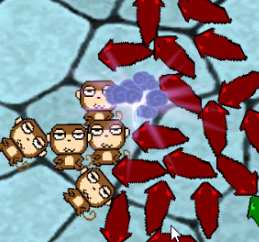
\includegraphics[width=\textwidth]{figures/NormalAttack.png}
        \caption{Saruによる通常攻撃}
        \label{fig:NormalAttack}
    \end{minipage}
    \hfill
    \begin{minipage}{0.45\textwidth}
        \centering
        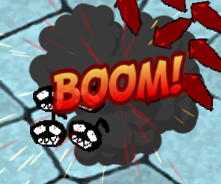
\includegraphics[width=\textwidth]{figures/ExplosionAttack.png}
        \caption{Piroriによる爆発攻撃}
        \label{fig:ExplosionAttack}
    \end{minipage}
\end{figure}

また攻撃パターンを入れ替えてみても、正常に動作することが確認できた。



\subsubsection{Observerパターンの実装}
以下に、Observerパターンを用いたキャラクターの死亡イベントの実装を示す。
まず、PlayerCommandクラスの実装をリスト\ref{lst:PlayerCommand}に示す。
赤文字の部分が今回Observerパターンを適用するにあたって注目すべき部分である。
\begin{lstlisting}[language=CSharp, caption=PlayerCommandクラス, label={lst:PlayerCommand}]
using System;
using System.Collections.Generic;
using UnityEngine;
using UnityEngine.EventSystems;
using UniRx;
using UniRx.Triggers;

/// <summary>
/// キャラクターの選択とコマンドの発行を管理するスクリプト
/// </summary>
public class PlayerCommand : MonoBehaviour
{
    [SerializeField] private GameObject uiManager;
    private ButtonManagerScript buttonManagerScript;
    private ReactiveCollection<GameObject> selectedCharacters = new ReactiveCollection<GameObject>();
    private Dictionary<GameObject, IDisposable> characterSubscriptions = new Dictionary<GameObject, IDisposable>();
    private Vector3 destination;

    [SerializeField] private float selectionRadius = 2f;

    private void Start()
    {
        buttonManagerScript = uiManager.GetComponent<ButtonManagerScript>();

        // 左クリックでキャラクター選択または移動先の設定
        this.UpdateAsObservable()
            .Where(_ => Input.GetMouseButtonDown(0) && !EventSystem.current.IsPointerOverGameObject())
            .Where(_ => buttonManagerScript.SelectedButtonType.Value == ButtonType.None)
            .Subscribe(_ => ProcessMouseClick())
            .AddTo(this);

        // 右クリックで他のキャラクターの選択を解除
        this.UpdateAsObservable()
            .Where(_ => Input.GetMouseButtonDown(1))
            .Subscribe(_ => buttonManagerScript.ResetOther())
            .AddTo(this);
    }

    /// <summary>
    /// マウスクリック時の処理
    /// キャラクター選択または移動先の設定を行うメソッド
    /// </summary>
    private void ProcessMouseClick()
    {
        Vector3 mousePosition = Input.mousePosition;
        mousePosition.z = Camera.main.nearClipPlane;
        Vector3 worldPosition = Camera.main.ScreenToWorldPoint(mousePosition);
        worldPosition.z = 0;

        // 選択されたキャラクターがいない場合、選択範囲内のキャラクターを選択
        if (selectedCharacters.Count == 0)
        {
            SelectCharactersInRadius(mousePosition, worldPosition);
            return;
        }

        // 選択されたキャラクターがいる場合、移動先を設定
        destination = worldPosition;
        foreach (GameObject character in selectedCharacters)
        {
            if (character == null || !character) continue;

            PlayerMovement mover = character.GetComponent<PlayerMovement>();
            if (mover != null)
            {
                mover.SetDestination(destination);
            }

            // 選択解除時にスプライトを非表示にする
            var indicator = character.GetComponent<SelectionIndicator>();
            if (indicator != null)
            {
                indicator.Hide();
            }
        }

        selectedCharacters.Clear();
    }

    /// <summary>
    /// クリック位置付近のキャラクターを選択して停止させるメソッド
    /// </summary>
    private void SelectCharactersInRadius(Vector3 mousePosition, Vector3 worldPosition)
    {
        //selectionIndicator.Show(mousePosition);

        GameObject[] characters = GameObject.FindGameObjectsWithTag("Player");
        foreach (GameObject character in characters)
        {
            float distance = Vector3.Distance(character.transform.position, worldPosition);
            if (distance > selectionRadius) continue;

            Status status = character.GetComponent<Status>();
            if (status == null) continue;

            selectedCharacters.Add(character);

            // 選択されたキャラクターのスプライトを表示
            var indicator = character.GetComponent<SelectionIndicator>();
            if (indicator != null)
            {
                indicator.Show();
            }

            // 選択範囲内のキャラクター数の変化を把握するために死亡イベントを購読
            if (!characterSubscriptions.ContainsKey(character))
            {
                (*@\textcolor{red}{var subscription = status.OnDie}@*)
                    (*@\textcolor{red}{.Subscribe(\_ =>\{ }@*)
                        (*@\textcolor{red}{selectedCharacters.Remove(character);}@*)
                        (*@\textcolor{red}{Debug.Log("キャラクターが死んだため、selectedCharactersから削除しました。");}@*)
                        (*@\textcolor{red}{characterSubscriptions.Remove(character);}@*)
                    (*@\textcolor{red}{\})}@*)
                    (*@\textcolor{red}{.AddTo(this);}@*)

                characterSubscriptions[character] = subscription;
            }

            //キャラクターを停止
            Rigidbody2D rb = character.GetComponent<Rigidbody2D>();
            if (rb == null) continue;
            rb.velocity = Vector2.zero;

            status.SetState(PlayerState.Selected);
        }
    }
}

\end{lstlisting}

このコードは、Observerパターンを用いてキャラクターの死亡イベントを監視し、
適切な処理を実行する仕組みを実装している。まず、status.OnDie を購読することで、
キャラクターが死亡したときに通知を受け取る準備をする。OnDie はキャラクターの死亡時に発火する
イベントであり、これを購読することで、死亡時に実行する処理を事前に登録することができる。

次に、Subscribe を使用して、OnDie が発生した際の処理を指定する。
まず、死亡したキャラクターを選択中のキャラクターリストから削除する。
これは、プレイヤーが操作可能なキャラクターのリストから、死亡したキャラクターを適切に
除外するために行われる。その後、デバッグ用のログを出力し、キャラクターが削除されたことを記録する。
さらに、キャラクターごとに保持されていた購読情報を削除し、不要なイベントの購読を解除する。
これにより、死亡したキャラクターに関する処理が不要になったときに、適切にクリーンアップを
行うことができる。
最後に、AddTo(this) を呼び出し、購読を現在のオブジェクトに紐づける。
これによって、オブジェクトが破棄された際に購読も自動的に解除されるため、
不要なイベント購読が残ることによるメモリリークを防ぐことができる。


次に、Statusクラスの実装をリスト\ref{lst:ObserverStatus}に示す。
赤文字の部分が今回Observerパターンを適用するにあたって注目すべき部分である。
\begin{lstlisting}[language=CSharp, caption=ObserverパターンにおけるStatusクラス, label={lst:ObserverStatus}]

using System;
using System.Collections;
using UnityEngine;
using UniRx;

/// <summary>
/// キャラクターのステータスを管理するクラス
/// </summary>
public class Status : MonoBehaviour, IStatus
{

    private int hp;
    public int Hp
    {
        get => hp;
        private set
        {
            hp = value;
            if (hp <= 0)
            {
                Die();
            }
        }
    }

    private int attack;
    public int Attack
    {
        get => attack;
        private set => attack = value;
    }

    // キャラクターが死んだことを通知するイベント
    (*@\textcolor{red}{public IObservable<Unit> OnDie => onDie; }@*)
    (*@\textcolor{red}{private Subject<Unit> onDie = new Subject<Unit>(); }@*)

    /// <summary>
    /// ダメージを受けるメソッド
    /// </summary>
    public virtual void TakeDamage(int amount, string attackerTag)
    {
        Hp -= amount;
    }

    (*@\textcolor{red}{protected virtual void Die()}@*)
    (*@\textcolor{red}{\{}@*)
        (*@\textcolor{red}{Instantiate(deadEffect, transform.position, Quaternion.identity);}@*)
        (*@\textcolor{red}{onDie.OnNext(Unit.Default); // 死亡イベントを発行}@*)
        (*@\textcolor{red}{onDie.OnCompleted(); // イベントの完了を通知}@*)
        (*@\textcolor{red}{Destroy(gameObject);}@*)
    (*@\textcolor{red}{\}}@*)

}
\end{lstlisting}
このコードは、キャラクターの死亡イベントを Observer パターンを用いて管理する仕組みを実装している。
OnDieプロパティはIObservable<Unit>型として定義され外部から購読可能だが、
Subject<Unit>のonDieはprivateであり、外部から直接イベントを発行できない。
これにより、死亡イベントの発火はStatusクラス内でのみ行われる。

キャラクターがダメージを受けてHPが0以下になると Dieメソッドが呼ばれる。
このメソッドでは、Instantiateにより死亡エフェクトを表示し、onDie.OnNext(Unit.Default)
によって購読者に死亡イベントを通知する。続いて onDie.OnCompletedを実行し、
イベントの購読が完了したことを示す。最後にDestroy(gameObject)を呼び出してキャラクターを
ゲーム内から削除する。

この設計により、死亡イベントを購読しているPlayerCommandクラスなどが通知を受け取り、
適切な処理を実行できる。

以上のように、Observerパターンを用いることで、
キャラクターの死亡に伴う処理を他のクラスと疎結合に管理できるようになる。

\section{考察}
授業内で挙がった抽象クラス不要論について考える。
JavaやC\#などの言語では、インターフェースにデフォルト実装を持たせることができる。
共通のメソッドなどをインターフェースに定義しておくことで、同じ処理を
複数のクラスで実装する必要がなくなり、コードの重複を防ぐことができる。
コードの重複を防ぐことによって、保守性を高めることができる。
他にも、JavaやC\#などの言語では単一クラスしか実装継承できないが、
インターフェースを使うことで複数のインターフェースを実装することができる。
またインターフェースのデフォルト実装では、メソッドをオーバーライドすることができるため、
抽象クラスよりもすべての点においてインターフェースのほうが優れているように思える。

しかし抽象クラスとインターフェースの異なる点として、
まずUnityにおいては、ゲーム内のオブジェクトはすべてMonoBehaviourを継承している必要がある。
そのため、もし抽象クラスを使わずにインターフェースだけで実装しようとすると、
インターフェースはMonoBehaviourを継承することができないため、ゲーム内で
プログラムを動作させることができない。
そのため、Unityにおいては仕様継承と実装継承の両方を使うことができる抽象クラスが有用である。

また、抽象クラスはインターフェースと異なり、フィールドやコンストラクタを持つことができる。
そのため、インターフェースだけでは実装できない処理を抽象クラスで実装することができる。
今回の例では、抽象クラスCharacterBaseはIAttackBehavior型のインスタンス変数を持ち、
その中身を変更することで攻撃パターンを変更することができる。

このように、抽象クラスはインターフェースにない特性を持っているため、
状況によっては抽象クラスを使うことが有用であると考える。


\section{まとめ}
本レポートでは、ソフトウェアアーキテクチャ特論の授業で学んだ知識をもとに、
Webアプリケーションとゲームの両方に適用した事例を整理した。
具体的には、Ruby on Railsを用いたn年日記の開発と、
Unityを用いた2Dアクションゲームの設計と実装について述べた。
n年日記の開発では、RailsのMVCアーキテクチャを活用し、
データベース管理やマイグレーション機能を駆使して効率的な開発を行った。
ゲーム開発においては、StrategyパターンとObserverパターンを適用し、
キャラクターの攻撃パターンや死亡イベントの管理を実装した。
これにより、コードの再利用性と拡張性を向上させ、柔軟な設計を実現した。
今後の課題としては、さらなる設計パターンの学習と適用を通じて、
より高度なソフトウェアアーキテクチャの理解を深めることである。
この授業で得た知識と経験を基に、今後も継続的に学習を続け、技術力を向上させていきたい。

\section{参考文献}
\begin{thebibliography}{9}

    % \bibitem{article1} 
    % 著者名, 「論文タイトル」, 雑誌名, 巻(号), ページ, 出版年.

    \bibitem{website1} 
    10年日記, https://web.10nikki.com/welcome, 2025/02/21閲覧.
    \bibitem{website2}
    Rails MVCについて復習, https://zenn.dev/goldsaya/articles/2e7b501538007a, 2025/02/21閲覧.
    \bibitem{book1} 
    Eric Freeman, Elisabeth Robson 著, 佐藤 直生 監訳, 木下 哲也 訳, "Head Firstデザインパターン 第2版 ―頭とからだで覚えるデザインパターンの基本", オライリージャパン, 2022.
\end{thebibliography}

\end{document}